\section{Grundlagen}

\subsection{Grundbegriffe}

\begin{defi}{Feature Vector}
    Ein \emph{Feature Vector} fasst die (numerisch) parametrisierbaren Eigenschaften eines Musters in vektorieller Weise zusammen.

    Verschiedene, für das Muster charakteristische Merkmale, bilden die verschiedenen Dimensionen dieses Vektors.

    Die Gesamtheit der möglichen Merkmalsvektoren nennt man den \emph{Feature Space}.

    Merkmalsvektoren erleichtern eine automatische Klassifikation, da sie die zu klassifizierenden Eigenschaften stark reduzieren.\footnote{Statt eines kompletten Bildes muss zum Beispiel nur ein Vektor aus 10 Zahlen betrachtet werden.}
\end{defi}

\begin{defi}{Target Function}
    Eine Funktion $f: \mathcal{X} \to \mathcal{Y}$ heißt \emph{Target Function}, wobei $\mathcal{X}$ einen Feature Space und $\mathcal{Y}$ einen Label Space darstellt.

    $f$ ist dabei eine \emph{unbekannte} (\enquote{perfekte}) \emph{Funktion}, die für jeden Feature Vector $\mathbf{x}_i \in \mathcal{X}$ ein Label $y_i \in \mathcal{Y}$ liefert.
\end{defi}

\begin{example}{Feature Vector und Target Function}

    \begin{center}
        \begin{tikzpicture}[
            %  -{Stealth[length = 2.5pt]},
            start chain = going {right=of \tikzchainprevious.north east},
            FeatureBlock/.style={minimum width=2em, minimum height=2em, outer sep=0pt, on chain},
            LabelBlock/.style={minimum height=12em, outer sep=0pt, on chain},
            every node/.style={draw, label distance=0.5em},
            every on chain/.style={anchor=north west},
            node distance=10em
            ]
            {
            \node [FeatureBlock, label={[align=center]above left:{Eigenschaften (Features) des Kunden: \\ \hl{Feature Vector} $\mathbf{x}$}}, label=left:{Alter}] (x0) {};
            \node [LabelBlock, label={[align=center]above:{Entscheidung: \\ \hl{Label} $y$}}, text width=8em, align=center] (y) {Kredit gewähren: Ja (1), Nein (-1)};

            { [continue chain = going {below=of \tikzchainprevious.south west}, node distance=0]
            \chainin (x0);
            \node [FeatureBlock, label=left:{Familienstand}] (x1) {};
            \node [FeatureBlock, label=left:{Höhe nicht zurückgezahlter Kredite}] (x2) {};
            \node [FeatureBlock, label=left:{Geschlecht}] (x3) {};
            \node [FeatureBlock, label=left:{Aufenthaltsdauer am Wohnsitz}] (x4) {};
            \node [FeatureBlock, label=left:{Jahresgehalt}] (x5) {};
            }

            \path[->] ([xshift=2ex]x3.north east) edge node[above, draw=none]{\hl{Target Function} $f$} ([xshift=-2ex]y.west);
            %\draw[->] (x3.north east) +(2em,0) -- (y.west) node [midway, above, draw=none] {Funktion $f$};
            }
        \end{tikzpicture}
    \end{center}

\end{example}

\begin{defi}{Datensatz}
    Ein Datensatz $\mathcal{D}$ besteht aus einer Menge von Input-Output-Paaren $(\mathbf{x}_1, y_1), \ldots, (\mathbf{x}_N, y_N)$, die durch die unbekannte Target Function $f$ mit $y_i = f(\mathbf{x}_i)$ erzeugt wurden.
\end{defi}

\begin{defi}{Lernalgorithmus}
    Ein Lernalgorithmus $\mathcal{A}$ selektiert mithilfe der Daten $\mathcal{D}$ aus einer Menge von Kandidatenfunktionen die Funktion $g$, die $f$ am besten approximiert.

    Der Algorithmus $\mathcal{A}$ selektiert $g$, so dass $g(\mathbf{x}_i) \approx f(\mathbf{x}_i)$ für alle $(\mathbf{x}_i, y_i) \in \mathcal{D}$.
\end{defi}

\begin{defi}{Kandidatenfunktionen}
    Die Menge der \emph{Kandidatenfunktionen} (bzw. Hypothesen-Set) $\mathcal{H}$ beschreibt alle Funktionen, die zur Approximation einer Funktion $f$ benutzt werden können.

    Die Hypothese $g \in \mathcal{H}$ mit $g(\mathbf{x}_i) \approx f(\mathbf{x}_i)$ wird dann \emph{finale Hypothese} genannt.
\end{defi}

\begin{defi}{Lernmodell}
    Ein \emph{Lernmodell} besteht aus einem Lernalgorithmus $\mathcal{A}$ und einer Menge von Kandidatenfunktionen bzw. dem Hypothesen-Set $\mathcal{H}$.
\end{defi}

\begin{bonus}{Darstellung des Lernproblems}
    \begin{center}
        % https://tex.stackexchange.com/a/224623/243801
        \begin{tikzpicture}
            [myBox/.style={rectangle,
                        draw,
                        align=center,
                        inner sep=2.5mm}]

            \node[myBox, fill=blue!20] (unknownTargetFunction) at (-4, 4) {Unbekannte Target Function\\$f: \mathcal{X} \rightarrow \mathcal{Y}$};
            \node[myBox, fill=blue!20] (trainingExamples) at (-4, 2) {Trainingsdaten\\$\mathcal{D} = (\mathbf{x}_1,y_1),...,(\mathbf{x}_n,y_n)$};
            \node[myBox, fill=blue!20] (learningAlgorithm) at ( 0, 0) {Lernalgorithmus\\$\mathcal{A}$};
            \node[myBox, fill=blue!20] (finalHypothesis) at ( 5, 0) {Finale Hypothese\\$g \approx f$};
            \node[myBox, fill=blue!20] (hypothesisSet) at (-4,-2) {Hypothesenset\\$\mathcal{H}$};

            \draw [->] (unknownTargetFunction) to (trainingExamples);
            \draw [->] (trainingExamples) to [bend right] (learningAlgorithm.170);
            \draw [->] (hypothesisSet) to [bend left] (learningAlgorithm.190);
            \draw [->] (learningAlgorithm) to (finalHypothesis);

            \node[draw,dashed,red,inner sep=2mm,label={[text=red]below:Lernmodell},fit=(learningAlgorithm) (hypothesisSet)] {};
        \end{tikzpicture}
    \end{center}
\end{bonus}

\begin{defi}{Supervised Learning}
    Beim \emph{Supervised Learning} bzw. \emph{Predictive Learning} wird eine unbekannte Target Function $f: \mathcal{X} \to \mathcal{Y}$ mithilfe einer Menge von Input-Output-Paaren $(\mathbf{x}_1, y_1), \ldots, (\mathbf{x}_N, y_N)$ mit einer Funktion $g$ approximiert.
\end{defi}

\begin{defi}{Unsupervised Learning}
    Beim \emph{Unsupervised Learning} bzw. \emph{Descriptive Learning} wird eine unbekannte Funktion $f$ gesucht, die gegebene Daten $(\mathbf{x}_1, \ldots, \mathbf{x}_N)$ gut beschreibt.
\end{defi}

\begin{defi}{Reinforcement Learning}
    Beim \emph{Reinforcement Learning} bzw. \emph{Reinforcement Learning} wird eine unbekannte Strategie $S$ gesucht, die eine Belohnung maximiert.

    Dabei wird zu jedem Input ein möglicher Output berechnet und bewertet.
    $\pi$ ist dann die Funktion, die die unbekannte beste Strategie $S$ approximiert.
\end{defi}

\begin{defi}{Perzeptron}
    Das \emph{Perzeptron} ist ein vereinfachtes künstliches neuronales Netz, das  in der Grundversion (einfaches Perzeptron) aus einem einzelnen künstlichen Neuron mit anpassbaren Gewichtungen $w_1, \ldots, w_d$ und einem Schwellenwert (Bias) besteht.

    Sei $\mathbf{w} = \vektor{w_1 & \ldots & w_d}^T$ ein Gewichtsvektor und $\mathbf{x} = \vektor{x_1 & \ldots & x_d}^T$ ein Feature Vector.

    Ziel des Perzeptrons ist es dann, einem Feature Vector $\mathbf{x}$ einen binären Output $h(\mathbf{x})$ zu zuzuweisen.
    Es gilt die \emph{Perzeptron-Gleichung}:
    \[
        h(\mathbf{x}) = \sign(\mathbf{w}^T\mathbf{x}), \ \text{mit} \ w_0 = 1, \, x_0 = 1
    \]

    % https://tex.stackexchange.com/a/132471/243801
    \begin{center}
        \begin{tikzpicture}[
                init/.style={
                        draw,
                        circle,
                        inner sep=2pt,
                        font=\Huge,
                        join = by -latex
                    },
                squa/.style={
                        draw,
                        inner sep=2pt,
                        font=\Large,
                        join = by -latex
                    },
                start chain=2,node distance=13mm
            ]
            \node[on chain=2]
            (x2) {$x_2$};
            \node[on chain=2,join=by {Circle[open]}-latex]
            {$w_2$};
            \node[on chain=2,init] (sigma)
            {$\displaystyle\Sigma$};
            \node[on chain=2,squa,label=below:{\parbox{2cm}{\centering \tiny Aktivierungs- \\ funktion}}]
            {$h$};
            \node[on chain=2,label=below:{\tiny Output},join=by -latex]
            {$y$};
            \begin{scope}[start chain=1]
                \node[on chain=1] at (0,1.5cm)
                (x1) {$x_1$};
                \node[on chain=1,join=by {Circle[open]}-latex]
                (w1) {$w_1$};
            \end{scope}
            \begin{scope}[start chain=3]
                \node[on chain=3,label=below:{\tiny Inputs}] at (0,-1.5cm)
                (x3) {$x_3$};
                \node[on chain=3,label=below:{\tiny Gewichte},join=by {Circle[open]}-latex]
                (w3) {$w_3$};
            \end{scope}
            \node[label=above:\parbox{2cm}{\centering {\tiny Bias} \\ $b$}] at (sigma|-w1) (b) {};

            \draw[-latex] (w1) -- (sigma);
            \draw[-latex] (w3) -- (sigma);
            \draw[{Circle[open]}-latex] (b) -- (sigma);

            %\draw[decorate,decoration={brace,mirror}] (x1.north west) -- node[left=10pt] {Inputs} (x3.south west);
        \end{tikzpicture}
    \end{center}
\end{defi}

\begin{bonus}{Perzeptron-Gleichung (Herleitung)}
    Es soll gelten:
    \[
        h(\mathbf{x}) =
        \begin{cases}
            1, \quad  & \text{wenn} \ \displaystyle \sum_{i=1}^d w_i x_i > \text{Schwellenwert} \\
            -1, \quad & \text{wenn} \ \displaystyle \sum_{i=1}^d w_i x_i < \text{Schwellenwert}
        \end{cases}
    \]

    Wir formen um und erhalten:
    \begin{alignat*}{2}
                     & \sum_{i=1}^d w_i x_i                 &  & > -b \qquad (b := -\text{Schwellenwert}) \\
        \equiv \quad & \sum_{i=1}^d w_i x_i + 1 \cdot b     &  & > 0                                      \\
        \equiv \quad & \sum_{i=1}^d w_i x_i + x_0 \cdot w_0 &  & > 0 \qquad (x_0 := 1, w_0 := b)          \\
        \equiv \quad & \sum_{i=0}^d w_i x_i                 &  & > 0                                      \\
        \equiv \quad & \mathbf{w}^T \mathbf{x}              &  & > 0
    \end{alignat*}

    Damit gilt direkt:
    \[
        h(\mathbf{x}) = \sign(\mathbf{w}^T\mathbf{x}), \ \text{mit} \ w_0 = 1, \, x_0 = 1
    \]
    \qed
\end{bonus}

\begin{bonus}{Perzeptron-Geradengleichung}
    Für $d = 2$ definiert der Gewichtsvektor $\mathbf{w} = \vektor{w_0 & w_1 & w_2}^T$ eine Gerade durch:
    \[
        x_2 = - \frac{w_1}{w_2} x_1 + \frac{w_0}{w_2} = m x_1 + b
    \]
\end{bonus}

\begin{defi}{Perzeptron Lern-Algorithmus}
    Der \emph{Perzeptron-Lern-Algorithmus} verändert den Gewichtsvektor $\mathbf{w}$ so lange, bis die Daten durch die durch $\mathbf{w}$ definierte Hyperebene komplett linear separiert sind.

    Der Algorithmus terminiert nicht, wenn die Daten nicht linear separiert sind.
\end{defi}

\begin{defi}{Pocket-Algorithmus}
    Der \emph{Pocket-Algorithmus} führt einen Lernschritt mithilfe des Perzeptron-Lern-Algorithmus (PLA) durch und prüft, ob der In-Sample-Fehler nach dem Lernschritt kleiner geworden ist.
    Falls dem so ist, merkt sich der Pocket-Algorithmus das (er \enquote{steckt den Gewichtsvektor des Perzeptron in seine Tasche} (engl. \emph{pocket})) und führt den nächsten PLA-Schritt durch.
    Wenn der Prozess am Ende abgebrochen wird, befindet sich in seiner Tasche der Gewichtsvektor (und damit die Gerade), die die Daten am besten (d.h. mit kleinstem In-Sample-Fehler) separiert.

    Der Algorithmus ist wie folgt:

    Sei $\mathbf{\hat{w}}$ der Gewichtsvektor des Pocket-Algorithmus.
    Sei $t$ eine Laufvariable, die von $0$ bis $(T-1)$ läuft.
    Sei $\mathbf{{w}}^{(t)}$ der Gewichtsvektor von PLA zum Iterationsschritt $t$.
    \begin{enumerate}
        \item Setze $\mathbf{\hat{w}}=\mathbf{w}^{(0)}=\mathbf{0}$. Setze den In-Sample Fehler $E_{\text{in}}(\mathbf{\hat{w}}) = 1$.
        \item Für $t=0,\ldots,T-1$, führe aus:
              \begin{enumerate}
                  \item Starte PLA mit $\mathbf{w}^{(t)}$ und lasse PLA ein einziges Gewichtsupdate durchführen. Erhalte $\mathbf{w}^{(t+1)}$.
                  \item Ermittle den In-Sample Fehler $E_{\text{in}}(\mathbf{w}^{(t+1)})$ für den Trainingsdatensatz.
                  \item Wenn $E_{\text{in}}(\mathbf{w}^{(t+1)}) < E_{\text{in}}(\mathbf{\hat{w}})$, dann setze  $\mathbf{\hat{w}}=\mathbf{w}^{(t+1)}$
              \end{enumerate}
        \item Gebe $\mathbf{\hat{w}}$ zurück.
    \end{enumerate}
\end{defi}

\begin{defi}{Trainings- und Testset}
    Bei überwachten Lernverfahren wird ein gegebener Datensatz in der Regel in mindestens zwei verschiedene Datensätze unterteilt: \emph{Trainings-} und \emph{Testset}.

    Ein \emph{Trainingsset} ist ein Datensatz mit Beispielen, die für das Lernen der Muster und Zusammenhänge in den Daten verwendet wird.
    Die Anpassung der Gewichte des Algorithmus wird über das Trainingsset antrainiert d.h. der Algorithmus lernt aus diesen Daten.

    Das \emph{Testset} ist von dem Trainingsset unabhängig, sollte jedoch die gleiche Wahrscheinlichkeitsverteilung wie das Trainingsset aufweisen.
    Das Testset wird bei dem Training nicht genutzt d.h. der Algorithmus kennt die Daten nicht und kann diese nicht zum Lernen nutzen. Auch hier sind Beispiele bzw. Zielvariablen vorhanden, woran im Anschluss die Qualität des Modells gemessen werden kann.
\end{defi}

\begin{defi}{In-Sample Error}
    Der \emph{In-Sample Error} gibt an, wie viele Datenpunkte in einer Stichprobe falsch klassifiziert wurden.

    Es gilt:
    \[
        E_\text{in} = \frac{1}{N} \sum_{i=1}^N \llbracket h(\mathbf{x}_i) \neq f(\mathbf{x}_i) \rrbracket
    \]

    Der In-Sample Error ist leicht zu bestimmen, da er lediglich auf dem gegebenen Datensatz berechnet werden muss.
\end{defi}

\begin{defi}{Out-of-Sample Error}
    Der \emph{Out-of-Sample Error} gibt die Fehlerrate an, die eine Hypothese $h_1$ auf allen möglichen Datenpunkten macht.

    Es gilt:
    \[
        E_\text{out} = P[h_1(\mathbf{x}) \neq f(\mathbf{x})]
    \]

    Der Out-of-Sample Error ist im Allgemeinen nicht exakt bestimmbar, da die Zukunft nicht vorhersehbar ist.

    Stattdessen wird er auf einem speziellen \emph{Trainingsset} berechnet und damit geschätzt.
\end{defi}

\begin{bonus}{Darstellung des Lernproblems}

    \begin{center}
        % https://tex.stackexchange.com/a/224623/243801
        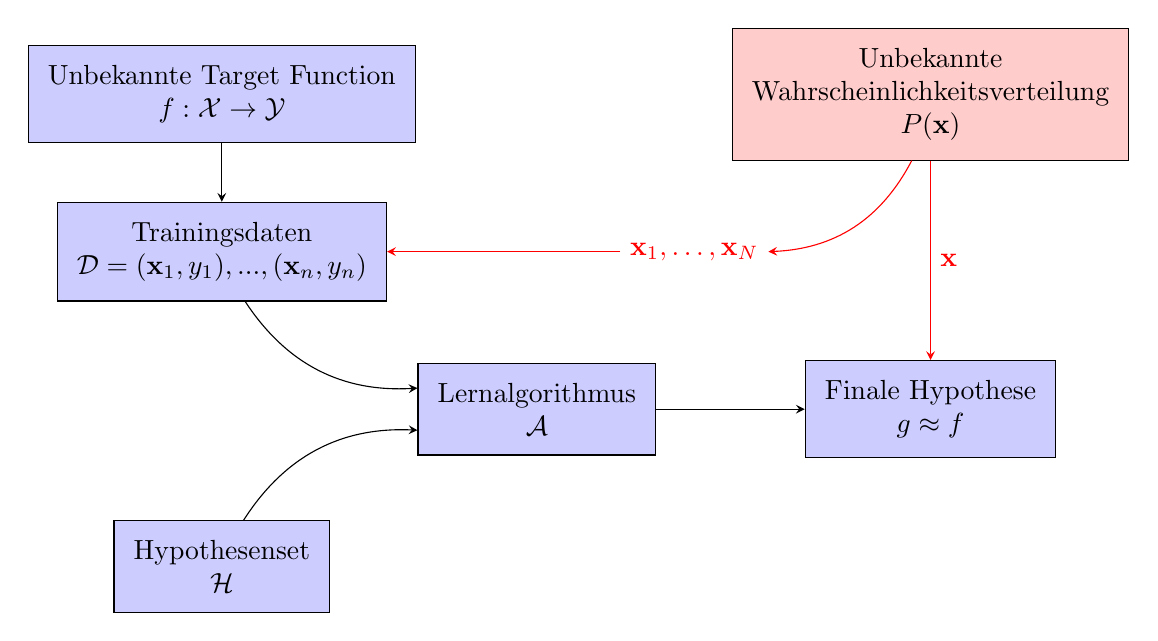
\begin{tikzpicture}
            [myBox/.style={rectangle,
                        draw,
                        align=center,
                        inner sep=2.5mm}]

            \node[myBox, fill=blue!20] (unknownTargetFunction) at (-4, 4) {Unbekannte Target Function\\$f: \mathcal{X} \rightarrow \mathcal{Y}$};
            \node[myBox, fill=blue!20] (trainingExamples) at (-4, 2) {Trainingsdaten\\$\mathcal{D} = (\mathbf{x}_1,y_1),...,(\mathbf{x}_n,y_n)$};
            \node[myBox, fill=blue!20] (learningAlgorithm) at ( 0, 0) {Lernalgorithmus\\$\mathcal{A}$};
            \node[myBox, fill=blue!20] (finalHypothesis) at ( 5, 0) {Finale Hypothese\\$g \approx f$};
            \node[myBox, fill=blue!20] (hypothesisSet) at (-4,-2) {Hypothesenset\\$\mathcal{H}$};

            \node[myBox, fill=red!20] (probabilityDistribution) at (5,4) {Unbekannte\\Wahrscheinlichkeitsverteilung\\$P(\mathbf{x})$};

            \node[red] (x) at (2, 2) {$\mathbf{x}_1, \ldots, \mathbf{x}_N$};

            \draw [->] (unknownTargetFunction) to (trainingExamples);
            \draw [->] (trainingExamples) to [bend right] (learningAlgorithm.170);
            \draw [->] (hypothesisSet) to [bend left] (learningAlgorithm.190);
            \draw [->] (learningAlgorithm) to (finalHypothesis);

            \draw [->, red] (probabilityDistribution) to [bend left] (x.east);
            \draw [->, red] (x) to (trainingExamples);
            \draw [->, red] (probabilityDistribution) to node [midway, right] {$\mathbf{x}$} (finalHypothesis) ;

            %\node[draw,dashed,red,inner sep=2mm,label={[text=red]below:Lernmodell},fit=(learningAlgorithm) (hypothesisSet)] {};
        \end{tikzpicture}
    \end{center}
\end{bonus}

\begin{defi}{Target Verteilung}
    Eine \emph{Target Verteilung} unterscheidet sich dahingehend von einer Target Function, dass sie nicht zwangsläufig deterministisch ist.

    Targets können zufällige Anteile haben (mit \emph{Rauschen} kontaminiert sein).
    Dann ist $y$ eine Zufallsvariable, die von $\mathbf{x}$ abhängt:
    \[
        y = P(y \mid \mathbf{x})
    \]

    Eine Target Function ist also eine deterministische Target Verteilung (also ohne Rauschen).

    Die Datenpunkte einer Target Verteilung entstehen durch Sampeln der multivariaten Verteilung
    \[
        P(\mathbf{x}, y) = P(\mathbf{x}) P(y \mid \mathbf{x})
    \]
\end{defi}

\begin{bonus}{Darstellung des Lernproblems}

    \begin{center}
        % https://tex.stackexchange.com/a/224623/243801
        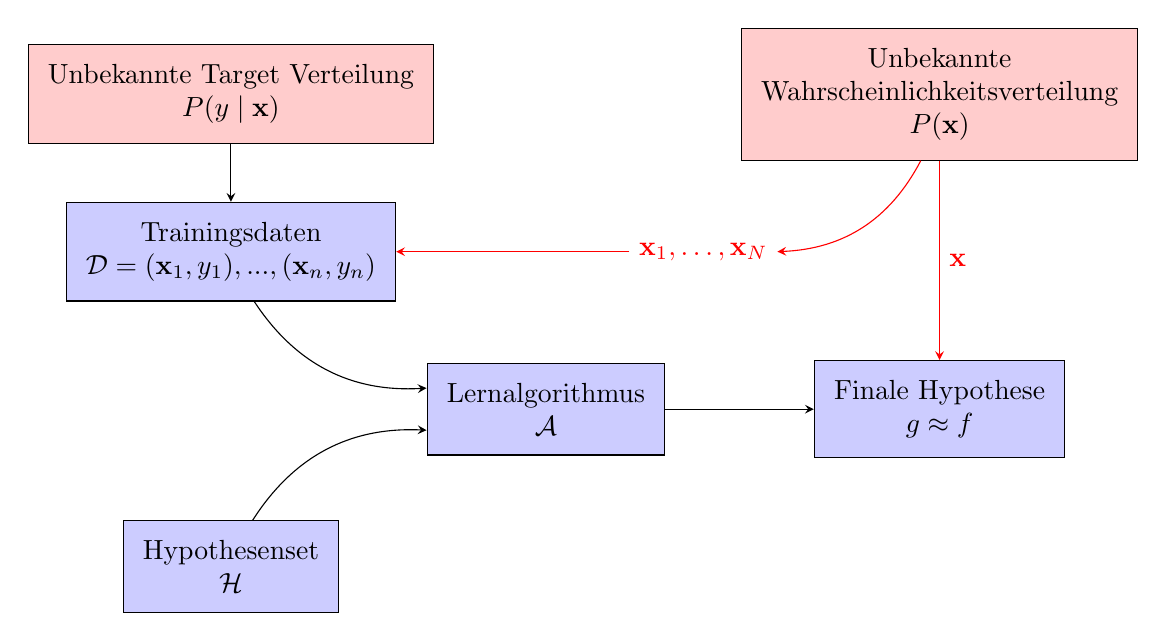
\begin{tikzpicture}
            [myBox/.style={rectangle,
                        draw,
                        align=center,
                        inner sep=2.5mm}]

            \node[myBox, fill=red!20] (unknownTargetDistribution) at (-4, 4) {Unbekannte Target Verteilung\\$P(y \mid \mathbf{x})$};
            \node[myBox, fill=blue!20] (trainingExamples) at (-4, 2) {Trainingsdaten\\$\mathcal{D} = (\mathbf{x}_1,y_1),...,(\mathbf{x}_n,y_n)$};
            \node[myBox, fill=blue!20] (learningAlgorithm) at ( 0, 0) {Lernalgorithmus\\$\mathcal{A}$};
            \node[myBox, fill=blue!20] (finalHypothesis) at ( 5, 0) {Finale Hypothese\\$g \approx f$};
            \node[myBox, fill=blue!20] (hypothesisSet) at (-4,-2) {Hypothesenset\\$\mathcal{H}$};

            \node[myBox, fill=red!20] (probabilityDistribution) at (5,4) {Unbekannte\\Wahrscheinlichkeitsverteilung\\$P(\mathbf{x})$};

            \node[red] (x) at (2, 2) {$\mathbf{x}_1, \ldots, \mathbf{x}_N$};

            \draw [->] (unknownTargetDistribution) to (trainingExamples);
            \draw [->] (trainingExamples) to [bend right] (learningAlgorithm.170);
            \draw [->] (hypothesisSet) to [bend left] (learningAlgorithm.190);
            \draw [->] (learningAlgorithm) to (finalHypothesis);

            \draw [->, red] (probabilityDistribution) to [bend left] (x.east);
            \draw [->, red] (x) to (trainingExamples);
            \draw [->, red] (probabilityDistribution) to node [midway, right] {$\mathbf{x}$} (finalHypothesis) ;

            %\node[draw,dashed,red,inner sep=2mm,label={[text=red]below:Lernmodell},fit=(learningAlgorithm) (hypothesisSet)] {};
        \end{tikzpicture}
    \end{center}

\end{bonus}

\subsection{Lineare Klassifikation und Regression}

\begin{defi}{Arten von Supervised Learning}
    Wir unterscheiden zwischen drei Arten des Supervised Learning, die sich in ihrer Target Function $f$ unterscheiden:
    \begin{itemize}
        \item \emph{Klassifikation}: $f$ bildet auf diskrete Klassen ab
        \item \emph{Regression}: $f$ bildet auf relle Zahlen ab
        \item \emph{Logistische Regression}: $f$ bildet auf Wahrscheinlichkeiten ab
    \end{itemize}
\end{defi}

\begin{defi}{Lineares Modell}
    \emph{Lineare Modelle} kombinieren Features linear miteinander:
    \[
        \theta (s(\mathbf{x})) = \theta \left( \sum_{i=0}^d w_i x_i \right) = \theta (\mathbf{w}^T \mathbf{x})
    \]

    Man unterscheidet zwischen:
    \begin{itemize}
        \item \emph{Lineare Klassifikation}:
              \begin{itemize}
                  \item $\theta$ bildet ab in verschiedene Klassen.
                  \item Beispiel: $\theta(\cdot) = \sign(\cdot)$
              \end{itemize}
        \item \emph{Lineare Regression}:
              \begin{itemize}
                  \item $\theta$ bildet ab in die reellen Zahlen.
                  \item Beispiel: $\theta(\cdot) = \id(\cdot) = \cdot$
              \end{itemize}
        \item \emph{Lineare Logistische Regression}:
              \begin{itemize}
                  \item $\theta$ bildet ab in die rellen Zahlen im Intervall $[0,1]$.
                  \item Beispiel: $\theta(\cdot) = \frac{e^s}{1+e^s}$ (Logistische Funktion)
              \end{itemize}
    \end{itemize}
\end{defi}

\begin{defi}{Lineare Regression}
    Die unbekannte Target Function sei eine bedingte Wahrscheinlichkeitsverteilung $P(y \mid x)$ statt einer deterministischen Target Function $y = f(\mathbf{x})$.

    Wir nehmen an, dass eine \emph{lineare Kombination} der Features $\mathbf{x}$ die Target Function approximiert.

    Die Datenpunkte sollten also möglichst wenig von einer optimalen Hypothese abweichen\footnote{Wir betrachten die quadratische Abweichung (\enquote{Methode der kleinsten Quadrate}).}.

    Dabei stammt $h(\mathbf{x})$ aus dem Hypothesenset $\mathcal{H}$ mit Hypothesen der Form:
    \[
        \mathcal{H}: h(\mathbf{x}) = \sum_{i=0}^d w_i x_i \ \text{mit} \ \mathbf{x} \in \{ 1 \} \times \R^d \ \text{und} \ w \in \R^{d+1}
    \]

    Out-of-Sample Error:
    \[
        E_\text{out}(h) = \Mean((h(\mathbf{x}) - y)^2)
    \]

    In-Sample Error (mit $\displaystyle \mathbf{X} = \vektor{\mathbf{x}_1^T \\ \ldots \\ \mathbf{x}_N^T} \in \R^{N\times (d+1)}$ und $\displaystyle \mathbf{y} = \vektor{y_1 \\ \ldots \\ y_N} \in \R^{N}$):
    \[
        E_\text{in}(\mathbf{w}) = \frac{1}{N} \sum_{i=1}^N ( \mathbf{w}^T \mathbf{x}_i) - y_i)^2 = \frac{1}{N} \cdot \norm{\mathbf{X} \mathbf{w} - \mathbf{y}}^2
    \]

    Gefunden werden soll also ein $\mathbf{w}$, sodass $E_\text{in}$ minimal ist.\footnote{$\mathbf{w}_\text{lin} = \arg\min_\mathbf{w} E_\text{in}(\mathbf{w})$}
    % \[
    %     \mathbf{w}_\text{lin} = \arg\min_\mathbf{w} E_\text{in}(\mathbf{w})
    % \]

    Es gilt (wobei $\mathbf{X}^\dagger$ die Pseudoinverse von $\mathbf{X}$ ist):
    \[
        \mathbf{w}_\text{lin} = \mathbf{X}^\dagger \mathbf{y} = (\mathbf{X}^T \mathbf{X})^{-1} \mathbf{X}^T \mathbf{y}
    \]
\end{defi}

\begin{defi}{Polynomielle Regression}
    Die \emph{polynomielle Regression} ist eine Form der Regressionsanalyse, bei der die Beziehung zwischen des Feature Vectors $\mathbf{x}$ und des Targets $y$ als Polynom $n$-ten Grades in $\mathbf{x}$ modelliert wird.
    Die polynomielle Regression passt eine nichtlineare Beziehung zwischen dem Wert von $\mathbf{x}$ und dem entsprechenden bedingten Mittelwert von $y$ an, bezeichnet als $\Mean(y \mid \mathbf{x})$.

    Obwohl die polynomiale Regression ein nichtlineares Modell an die Daten anpasst, ist sie als statistisches Schätzproblem linear in dem Sinne, dass die Regressionsfunktion $\Mean(y \mid \mathbf{X})$ linear in den unbekannten Parametern ist, die aus den Daten geschätzt werden.

    Aus diesem Grund wird die polynomiale Regression als ein Spezialfall der multiplen linearen Regression betrachtet.

    Der $\mathcal{Z}$-Raum ist dann der Feature Space der transformierten Variable $\Phi(x)$.
    Dabei ist $\Phi(x)$ eine Feature Transform, die $x$ als $\tilde{d}$-dimensionales Polynom modelliert.

    Es gilt also:
    \[
        \mathcal{Z}: \Phi(x) \in \{ 1 \} \times \R^{\tilde{d}}
    \]
\end{defi}

\subsection{Approximation versus Generalisierung}

\begin{defi}{Approximation}
    Das Ziel der \emph{Approximation} ist es, einen möglichst kleinen In-Sample Error $E_\text{in}$ auf dem Trainingsset zu erhalten.
\end{defi}

\begin{defi}{Generalisierung}
    Das Ziel der \emph{Generalisierung} ist es, einen Out-of-Sample Error $E_\text{out}$ zu erhalten, der annähernd dem In-Sample Error $E_\text{in}$ entspricht:
    \[
        E_\text{out}(h) \approx E_\text{in}(h)
    \]
\end{defi}

\begin{defi}{Approximations-Generalisierungsabwägung}
    Approximation und Generalisierung stehen im \emph{Konflikt}.

    In der Praxis ist oft entweder
    \begin{itemize}
        \item \emph{perfekte Approximation} und \emph{schlechte Generalisierung}, oder
        \item \emph{sehr gute Generalisierung} aber \emph{schlechte Approximation}
    \end{itemize}
    zu beobachten.

    Einflussfaktoren für diesen Konflikt sind beispielsweise:
    \begin{itemize}
        \item Komplexität des Lernmodells (Modellkomplexität)
        \item Anzahl der Trainingsdatenpunkte (Datenmenge)
        \item Kontamination der Daten mit Rauschen (Rauschkontamination)
    \end{itemize}
\end{defi}

\begin{bonus}{Approximations-Generalisierungsabwägung}
    Ergebnis der statistischen Lerntheorie:
    \[
        E_\text{out}(g) \leq E_\text{in}(g) + \Omega (N, \mathcal{H})
    \]
    Dabei ist $\Omega$ ein Strafterm, der eine hohe Modellkomplexität bestraft.

    \begin{center}
        % https://tex.stackexchange.com/a/563020/243801
        \tikzset{>=stealth,
            OptimumStyle/.style={align=center,anchor=east,rotate=90,font=\sffamily\scriptsize}
        }
        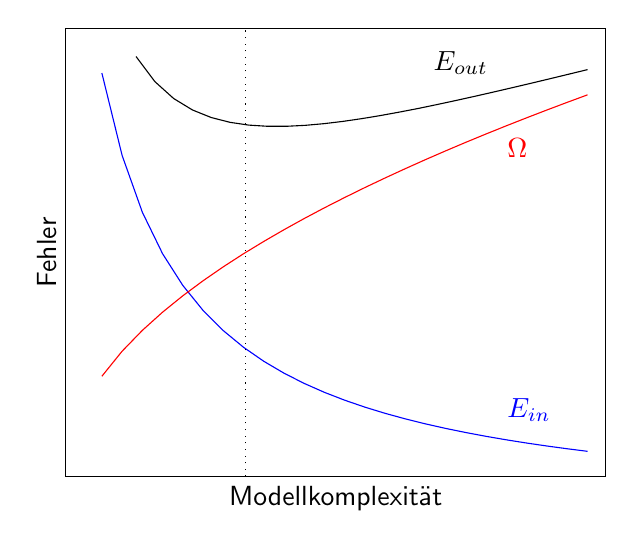
\begin{tikzpicture}[font=\sffamily]
            \begin{axis}[
                    xmin= 0,
                    xmax= 3,
                    ymin= 0,
                    ymax= 2,
                    xlabel=Modellkomplexität,
                    ylabel=Fehler,
                    ticks=none,
                    xticklabels={\empty},
                    yticklabels={\empty}
                ]
                \addplot[domain=0.2:2.9,blue] {1/(x+0.3)-0.2};   %In-Sample Error
                \addplot[domain=0.2:2.9,red] {x^(1/2)};   %Penalty
                \addplot[domain=0.39:2.9,black] {x^(1/2) + 1/(x+0.3)-0.2};  %Out-of-Sample Error
                \addplot[dotted,thin] coordinates {(1,0) (1,2)};       %Optimum model complexity
                %\node[OptimumStyle] at (axis cs:0.9,2) {optimale\\Modellkomplexität};
                \node[anchor=south west,text=blue] at (axis cs:2.4,0.2){$E_\text{in}$};
                \node[anchor=north west,text=red] at (axis cs:2.4,1.55){$\Omega$};
                \node[anchor=south east,align=center] at (axis cs:2.4,1.75){$E_\text{out}$};
                \legend{}
            \end{axis}
        \end{tikzpicture}
    \end{center}

    \begin{itemize}
        \item Links der optimalen Modellkomplexität findet \emph{Underfitting} statt.
        \item Rechts der optimalen Modellkomplexität findet \emph{Overfitting} statt.
    \end{itemize}
\end{bonus}

\begin{defi}{Bias}
    Für verschiedene Datensätze $\mathcal{D}$ desselben Lernproblems erhalten wir verschiedene finale Hypothesen $g$.

    Der \emph{Bias} bzw. die \emph{Verzerrung} misst die Abweichung zwischen der über allen möglichen Datensätzen gemittelten finalen Hypothese $g$ und der Target Function $f$.

    Er charakterisiert weiterhin, wie stark unser Lernmodell (Hypothesenset und Algorithmus) von der Target Function prinzipiell abweicht.
\end{defi}

\begin{defi}{Varianz}
    Die \emph{Varianz} misst, wie stark eine durch einen gewählen Datensatz $\mathcal{D}$ gewonnene finale Hypothese um die mittlere finale Hypothese streut.

    Sie kann als Instabilität des Lernmodells interpretiert werden.
    Instabilität zeigt sich in großen Reaktionen des Lernmodells auf kleine Variationen in Datensätzen.

    Wächst die Größe der Datensätze, wird die Varianz kleiner.
\end{defi}

\begin{bonus}{Visualisierung Bias, Varianz}
    % https://tex.stackexchange.com/a/307285/243801
    \begin{center}
        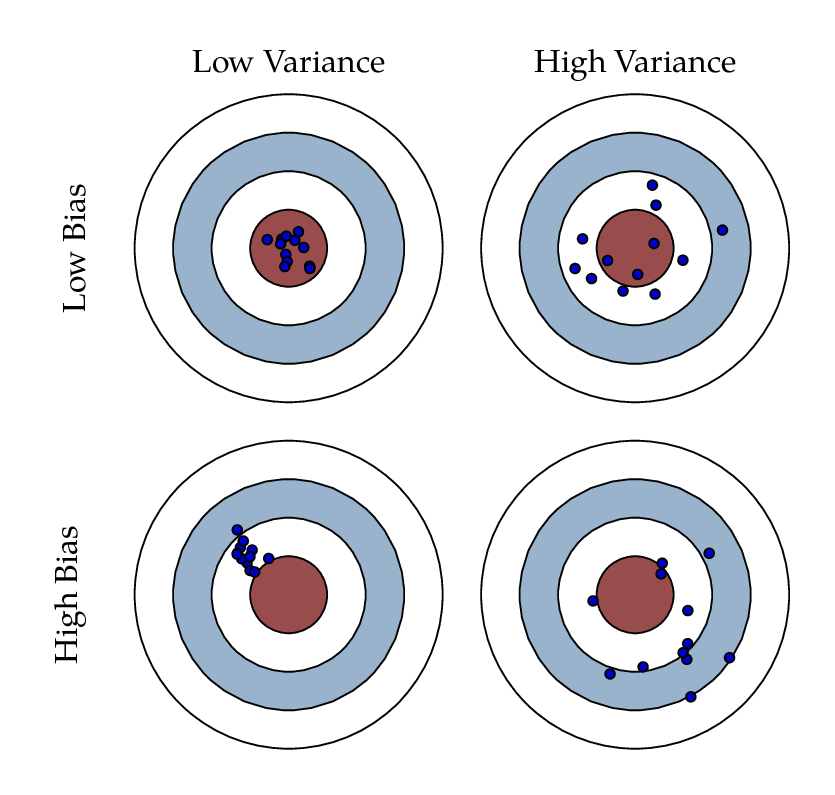
\includegraphics[width=.7\textwidth]{includes/figures/bonus_defi_variance.png}
    \end{center}
\end{bonus}

\begin{defi}{Bias-Variance Tradeoff}
    \begin{center}
        % https://tex.stackexchange.com/a/563020/243801
        \tikzset{>=stealth,
            OptimumStyle/.style={align=center,anchor=east,rotate=90,font=\sffamily\scriptsize}
        }
        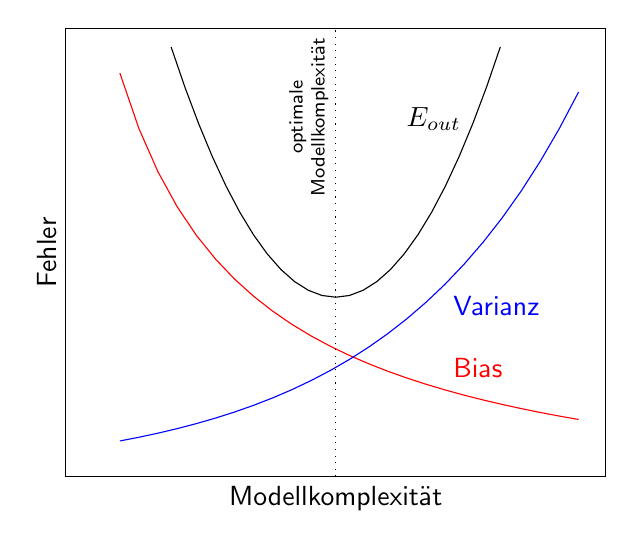
\begin{tikzpicture}[font=\sffamily]
            \begin{axis}[
                    xmin= 0,
                    xmax= 2,
                    ymin= 0,
                    ymax= 2,
                    xlabel=Modellkomplexität,
                    ylabel=Fehler,
                    ticks=none,
                    xticklabels={\empty},
                    yticklabels={\empty}
                ]
                \addplot[domain=0.2:1.9,red] {1/(x+0.3)-0.2};   %Bias
                \addplot[domain=0.2:1.9,blue] {0.12*e^(1.40*x)};   %Variance
                \addplot[domain=0.39:1.61,black] {3*(x-2)*x+3.8};  %Total error
                \addplot[dotted,thin] coordinates {(1,0) (1,2)};       %Optimum model complexity
                \node[OptimumStyle] at (axis cs:0.9,2) {optimale\\Modellkomplexität};
                \node[anchor=south west,text=red] at (axis cs:1.4,0.4){Bias};
                \node[anchor=north west,text=blue] at (axis cs:1.4,0.85){Varianz};
                \node[anchor=south east,align=center] at (axis cs:1.5,1.5){$E_\text{out}$};
                \legend{}
            \end{axis}
        \end{tikzpicture}
    \end{center}
\end{defi}

\begin{defi}{Overfitting}
    \emph{Overfitting} ist der Prozess, Hypothesen $h$ mit kleinerem In-Sample Error $E_\text{in}$ zu wählen, die zu wachsendem Out-of-Sample Error $E_\text{out}$ führen.

    Wir beobachten Overfitting für eine Hypothese $h$, wenn es eine weitere Hypothese $h'$ gibt, so dass gilt:
    \[
        E_\text{in}(h) \leq E_\text{in}(h') \ \text{aber} \ E_\text{out}(h) \geq E_\text{out}(h')
    \]

    Overfitting hängt davon ab, wie die gewählte Modellkomplexität zur Quantität und Qualität der Daten passt (und nicht, wie die gewählte Modellkomplexität zur Komplexität der Target Functionpasst).

    Es gilt:
    \begin{itemize}
        \item mehr Datenpunkte \emph{reduzieren} die Tendenz zu Overfitting
        \item mehr Rauschkontamination \emph{erhöht} die Tendenz zu Overfitting
        \item höhere Target Komplexität \emph{erhöht} die Tendenz zu Overfitting
    \end{itemize}
\end{defi}

\subsection{Regularisierung}

\begin{defi}{Regularisierung}
    \emph{Regularisierung} schränkt den Lernalgorithmus ein, um den Out-Of-Sample Error $E_\text{out}$ zu verbessern und Overfitting zu bekämpfen.\footnote{Aus einem ähnlichen Grund erfordert eine höhere Rauschkontamination auch eine stärkere Regularisierung.}

    Regularisierungstechniken sind meist heuristische Methoden;
    es fehlt oft eine mathematische Begründung, warum sie funktionieren.

    Aus dem bekannten Strafterm für Modellkomplexität in
    \[
        E_\text{out}(h) \leq E_\text{in} + \Omega(N, \mathcal{H}) \ \text{für alle} \ h \in \mathcal{H}
    \]
    sieht man:
    \begin{itemize}
        \item Wahl eines \emph{einfachen} Hypothesensets $\mathcal{H}$ verbessert die Schranke (geringere Modellkomplexität).
        \item Wahl einer \emph{einfachen Hypothese} $h \in \mathcal{H}$ verbessert die Schranke (Komplexität der Hypothese $\Omega(h)$ wird klein).
    \end{itemize}

    Regularisierung zielt darauf ab, einfache Hypothesen aus dem Hypothesenset zu wählen:
    \begin{itemize}
        \item Minimiere $E_\text{in}(h)$ und $\Omega(h)$ \emph{gleichzeitig}.
    \end{itemize}

    Regularisierung reduziert den Varianz-Term, doch der Bias-Term steigt an:
    \enquote{Wir tauschen den niedrigen Bias-Term gegen eine deutliche Verkleinerung des Varianz-Terms ein.}
    \footnote{Typisch für die Praxis: Nutzung eines komplexen Hypothesensets + Regularisierung ergibt die kleinsten Out-of-Sample Error $E_\text{out}$.}
\end{defi}

\begin{defi}{Augmented Error}
    Regularisierung kann durch den \emph{Augmented Error} bzw. \emph{erweiterten Fehler} $E_\text{aug}$ mit freiem Parameter $\lambda \geq 0$ stattfinden:
    \[
        E_\text{aug}(\mathbf{w}) = E_\text{in}(\mathbf{w}) + \frac{\lambda}{N} \underbrace{\mathbf{w}^T \mathbf{w}}_{\text{Strafterm} \ \Omega(h)}
    \]

    Dabei stellt das $\lambda$ ein, \enquote{wie stark} die Regularisierung sein soll.
    \footnote{
        Der Faktor $\nicefrac{1}{N}$ ist eingebaut, da mit mehr Datenpunkten weniger Regularisierung notwendig ist.
        Das ist nur eine Redefinition von $\lambda$.
    }

    Wir erwarten stärkere Regularisierung und bessere Generalisierung, wenn $\lambda$ ansteigt.
\end{defi}

\begin{defi}{Weight Decay}
    Das Ziel von \emph{Weight Decay} ist es, große Gewichte zu verhindern und dadurch \enquote{glattere} Hypothesen zu erzeugen.

    Explizit nutzen wir Weight Decay mit
    \[
        \Omega(h) = \mathbf{w}^T \mathbf{w}
    \]

    Insbesondere ist Rauschen auch meist \enquote{nicht glatt} bzw. hochfrequent.
    Dadurch schadet die Regularisierung mit Weight Decay dem Overfitting mehr als der Fähigkeit, das Signal in den Daten zu fitten.
\end{defi}

\begin{defi}{Lineare Regression mit Weight Decay}
    %Sei $\mathbf{Z} = \vektor{\mathbf{z}_1^T \\ \mathbf{z}_2^T \\ \vdots \\ \mathbf{z}_N^T}$.

    Lineare Regression ohne Regularisierung:
    \begin{itemize}
        \item Finde $\mathbf{w}_\text{lin}$, das $E_\text{in}$ minimiert:
              \[
                  E_\text{in}(\mathbf{w}) = \frac{1}{N} (\mathbf{Z}\mathbf{w} - \mathbf{y})^T (\mathbf{Z}\mathbf{w} - \mathbf{y})
              \]
              \[
                  \mathbf{w}_\text{lin} = \arg\min_\mathbf{w} E_\text{in}(\mathbf{w}) = (\mathbf{Z}^T \mathbf{Z})^{-1} \mathbf{Z}^T \mathbf{y}
              \]
    \end{itemize}

    Lineare Regression mit Regularisierung:
    \begin{itemize}
        \item Finde $\mathbf{w}_\text{aug}$, das $E_\text{aug}$ minimiert:
              \[
                  E_\text{aug}(\mathbf{w}) = E_\text{in}(\mathbf{w}) + \frac{\lambda}{N} \mathbf{w}^T \mathbf{w}
              \]
              \[
                  \mathbf{w}_\text{aug} = \arg\min_\mathbf{w} E_\text{aug}(\mathbf{w}) = (\mathbf{Z}^T \mathbf{Z} + \lambda \mathbf{I})^{-1} \mathbf{Z}^T \mathbf{y}
              \]
    \end{itemize}
\end{defi}

\subsection{Validierung}

\begin{defi}{Validierung}
    \emph{Validierungstechniken} werden genutzt
    \begin{itemize}
        \item zur Schätzung des Out-of-Sample Errors $E_\text{out}$
        \item zur Wahl von Modellen bzw. zur Bestimmung von Hyperparametern, z.B.
              \begin{itemize}
                  \item Parameter, die die Modellarchitektur bestimmen
                  \item Parameter, die den Lernalgorithmus betreffen
                  \item \emph{Regularisierungsparameter}
              \end{itemize}
    \end{itemize}
\end{defi}

\begin{bonus}{Lernkurve}
    \begin{center}
        \begin{tikzpicture}[font=\sffamily]
            \begin{axis}[
                    xmin= 0.4,
                    xmax= 5,
                    ymin= -2,
                    ymax= 2,
                    xlabel=Trainingsdatenpunktanzahl,
                    ylabel=Fehler,
                    ticks=none,
                    xticklabels={\empty},
                    yticklabels={\empty}
                ]
                \addplot[name path=Eout, domain=0.6:4.8,red] {1/x}; %E_out
                \addplot[name path=Ein, domain=0.6:4.8,blue] {-1/x}; %E_in

                \path[name path=axis, draw=none] (axis cs:0.6,-1.8) -- (axis cs:4.8,-1.8);

                % color between E_in and E_out
                \addplot[fill=red, fill opacity = 0.1, domain=0.6:4.8] fill between[of=Ein and Eout];
                \addplot[fill=blue, fill opacity = 0.1, domain=0.6:4.8] fill between[of=Ein and axis];
                \addplot[domain=0.6:4.8,black] {0}; %middle

                \node[anchor=south east,align=center, text=red] at (axis cs:4.5,0.5){$E_\text{out}$};
                \node[anchor=south east,align=center, text=blue] at (axis cs:4.5,-1){$E_\text{in}$};
                \legend{}
            \end{axis}
        \end{tikzpicture}
    \end{center}
\end{bonus}

\subsubsection{Schätzen des Out-of-Sample Errors}

\begin{defi}{Hold-Out Validierung (Schätzen des Out-of-Sample Errors)}
    Bei der \emph{Hold-Out Validierung} werden die Daten $\mathcal{D}$ zufällig in Trainingsset $\mathcal{D}_\text{train}$ ($N-K$ Datenpunkte) und Validierungsset $\mathcal{D}_\text{val}$ ($K$ Datenpunkte) aufgeteilt.
    \footnote{Typisch in der Praxis ist $K = \nicefrac{N}{5}$.}

    Die finale Hypothese $g^{-} \in \mathcal{H}$ wird dann auf dem Trainingsset erhalten.

    Der \emph{Validierungsfehler} $E_\text{val}$ wird dann mithilfe von $g^{-}$ auf dem Validierungsset $\mathcal{D}_\text{val}$ berechnet.

    Typisch ist folgendes Vorgehen:
    \begin{enumerate}
        \item Berechne Validierungsfehler und nutze $E_\text{val}$ als Schätzer für $E_\text{out}$.
        \item Bestimme finale Hypothese $g$ auf dem \emph{ganzen} Datensatz $\mathcal{D}$ (Retraining) und liefere $g$ aus.
    \end{enumerate}

    Hold-Out Validierung ist generell wenig rechenintensiv, da nur ein Modell trainiert werden muss.
\end{defi}

\begin{defi}{Leave-One-Out Kreuzvalidierung (LOO-CV) (Schätzen des Out-of-Sample Errors)}
    Bei der \emph{Leave-One-Out Kreuzvalidierung} (LOO-CV) werden die Daten $\mathcal{D}$ zufällig in Trainingsset mit $N-1$ Datenpunkten und Validierungsset mit einem Datenpunkt aufgeteilt.

    Sei $\mathcal{D}_n := \mathcal{D} \setminus (\mathbf{x}_n, y_n)$ und die auf $\mathcal{D}_n$ gelernte Hypothese $g^{-}_n \in \mathcal{H}$.

    Dann sei der punktweise Fehler auf dem Validierungsset $\{ \mathbf{x}_n, y_n \}$:
    \[
        e_n := E_\text{val}(g^{-}_n) = e(g^{-}_n(\mathbf{x}_n), y_n)
    \]

    Der gesamte Kreuzvalidierungsfehler $E_\text{CV}$ ist dann:
    \[
        E_\text{CV} = \frac{1}{N} \sum_{n=1}^N e_n
    \]

    Vorgehen:
    \begin{enumerate}
        \item Erzeuge $N$ Datensätze $\mathcal{D}_n$ aus dem Datensatz $\mathcal{D}$ mit $N$ Datenpunkten.
        \item Ermittle die finalen Hypothesen für jeden Datensatz $\mathcal{D}_n$.
        \item Erhalte den Kreuzvalidierungsfehler $E_\text{CV}$ als Mittelwert der Validierungsfehler $e_n$.
    \end{enumerate}

    LOO-CV ist generell sehr rechenintensiv, da $N$ Modelle trainiert werden müssen.
\end{defi}

\begin{defi}{V-fache Kreuzvalidierung (Schätzen des Out-of-Sample Errors)}
    Bei der \emph{V-fachen Kreuzvalidierung} werden die Daten $\mathcal{D}$ in $V$ gleich große disjunkte Teilmengen bzw. \emph{Folds} $\mathcal{D}_v$ aufgeteilt.
    Typische Werte für $V$ sind z.B. $5$ oder $10$.

    Für alle $v = 1, \ldots, V$ wird dann ein Modell auf $\mathcal{D} \setminus \mathcal{D}_v$ trainiert und der Validierungsfehler $E_v$ auf $\mathcal{D}_v$ berechnet.

    Der gesamte Kreuzvalidierungsfehler $E_\text{V-fold CV}$ ist dann:
    \[
        E_\text{V-fold CV} = \frac{1}{V} \sum_{v=1}^V E_v
    \]

    Von der Wahl von $V$ ist abhängig:
    \begin{itemize}
        \item Anzahl Datenpunkte im Trainingsset $N_\text{train} = \frac{V-1}{V} N$
        \item Anzahl Datenpunkte im Validierungsset $N_\text{val} = \frac{1}{V} N$
        \item Bias:
              \subitem kleines $V$
              \subitem $\implies$ $N_\text{train} \ll N$
              \subitem $\implies$ großer Bias für $E_\text{V-fold CV}$
              \subitem (Schätzer für $E_\text{out}$ bei $N_\text{train}$ Daten, interessieren uns aber für $N$ Daten)
        \item Varianz:
              \subitem großes $V$
              \subitem $\implies$ $N_\text{train} \approx N$ und $N_\text{val} \to 1$
              \subitem $\implies$ große Varianz für $E_\text{V-fold CV}$
              \subitem (verschiedene $g^{-}_n$ sind hochkorreliert, da Trainingsdaten fast identisch)
              \subitem $\implies$ Fehler $E_v$ sind stark korreliert.
    \end{itemize}
\end{defi}

\subsubsection{Modellauswahl}

\begin{defi}{Modellauswahl}
    Der wichtigste Anwendungsfall für Validierungstechniken ist die \emph{Modellauswahl} (\emph{model selection}) bzw. die Bestimmung von Hyperparametern.

    Die Idee:
    \begin{itemize}
        \item Nutze Validierung, um $E_\text{out}$ für \emph{mehrere Modelle} zu schätzen.
        \item Wähle das Modell mit der kleinsten Schätzung für $E_\text{out}$ aus.
    \end{itemize}

    Modelle können z.B. sein:
    \begin{itemize}
        \item Polynome mit unterschiedlicher Ordnung $Q$
        \item Ein Modell mit unterschiedlich starker Regularisierung $\lambda$: $(\mathcal{H}, \lambda_1), (\mathcal{H}, \lambda_2), \ldots, (\mathcal{H}, \lambda_M)$
    \end{itemize}
\end{defi}

\begin{defi}{Hold-Out Validierung (Modellauswahl)}
    Vorgehen:
    \begin{enumerate}
        \item Betrachte $M$ Modelle bzw. Hypothesensets $\mathcal{H}_1, \ldots, \mathcal{H}_M$
        \item Erhalte finale Hypothesen auf dem Trainingset: $g^{-}_1, \ldots, g^{-}_M$
        \item Errechne den Validierungsfehler $E_\text{val}$ als Schätzer für $E_\text{out}$ für jedes der $M$ Modelle:
              \[
                  E_\text{val}(m) = E_\text{val}(g^{-}_m), \, m \in 1, \ldots, M
              \]
        \item Selektiere bestes Modell $m^*$ mit dem kleinsten Validierungsfehler $E_m^*$
        \item Bestimme finale Hypothese $g$ des Modells $m^*$ auf dem ganzen Datensatz
    \end{enumerate}

    Der Validierungsfehler $E_\text{val}(g^{-}_m)$ wird zur Auswahl des finalen Modells genutzt und ist daher \enquote{optimistisch} verzerrt.
    Das hat zur Folge, dass der optimistische Validierungsfehler tendenziell niedriger ist als der wahre Out-of-Sample Error $E_\text{out}$.

    \emph{Wichtig}:
    Je mehr Lernentscheidungen über das Validierungsset getroffen werden, desto schlechter kann $E_\text{val}$ Aussagen über $E_\text{out}$ treffen und desto mehr wird das Validierungsset zum Traininsset.
\end{defi}

\begin{defi}{Leave-One-Out Kreuzvalidierung (LOO-CV) (Modellauswahl)}
    Vorgehen (bei der Auswahl des Regularisierungsparameters $\lambda$):
    \begin{enumerate}
        \item Definiere $M$ Modelle $(\mathcal{H}, \lambda_1), (\mathcal{H}, \lambda_2), \ldots, (\mathcal{H}, \lambda_M)$
        \item Bestimme für jedes Modell $m = 1, \ldots, M$ den Kreuzvalidierungsfehler $E_\text{CV}(m)$
        \item Selektiere bestes Modell $m^*$ mit dem kleinsten Kreuzvalidierungsfehler $E_\text{CV}$
        \item Nutze $(\mathcal{H}, \lambda_{m^*})$ und alle Daten $\mathcal{D}$, um die finale Hypothese $g_m^*$ zu trainieren.
    \end{enumerate}

    Insgesamt müssen hier also $(M \cdot N) + 1$ Modelle trainiert werden.
\end{defi}